\section{Experiment Definition}

\subsection{Goal}

The goal of the experiment is identified in Table  \ref{tab:msg1}, using the well-established
GQM goal definition pattern  \cite{Book:Exp}:

\begin{table}[h]                           
    \begin{tabular}{|c|c|}
    \hline

     \textbf{Analyze }   &   Performance Score                \\ \hline
     \textbf{For the purpose of} &   Evaluating correlation             \\ \hline          
     \textbf{With respect to their }    &   Energy Consumption  \\ \hline
     \textbf{From the point of view of}        &   Software Developers         \\ \hline
     \textbf{In the context of}   &   Web Apps           \\ \hline
     \multicolumn{2}{|c|}{\textbf{Result}} \\ \hline
     \multicolumn{2}{|c|}{\makecell{Analyze performance score for the purpose of evaluating how \\ performance correlates with respect to their energy consumption \\ from the point of view of software developers\\  in the context of Web Apps}} \\ \hline

    \end{tabular}
    \caption{Goal definition}
    \label{tab:msg1}                            

\end{table}

\subsection{Questions}

\textbf{[RQ1]}: \textit{To what extent do performance scores correlate to the energy consumption in the context of web apps?}
\newline

To answer this question we will randomly choose 21 web apps from the Alexa list of top visited web apps and load them on the device to measure the energy consumption of each\cite{Web:Alexa}. Then we will compare the energy consumption with the score obtained from Lighthouse and check whether there is any correlation between these two values or not.
\newline

\subsection{Metrics}

To answer the aforementioned questions and thus fulfill the objective of our experiment we will need the following metrics:
\newline

\begin{itemize}
	\item[--] Power consumption: measured in micro-watts.  It is the base metric that we will use to calculate energy consumption of different web apps.
   \item[--] Profiling time: The duration of each run of the experiment, based on the Time to interactive lightouse-metric for each web app in milliseconds
   	\item[--] Total energy consumption: It is measured in Joule based on power consumption over time to load the web application. This value is calculated using the following formula:
   	 \textit{Energy = Power x Time}   
   	 \newline
\end{itemize}


\subsection{GQM-Tree}

Figure \ref{fig:GQM} displays the visual representation of the GQM tree. This diagram illustrates how our experimental goal, the questions related to this goal and the metrics that are going to address those questions are derived from hierarchical model.
\newline

\begin{figure}[H]
  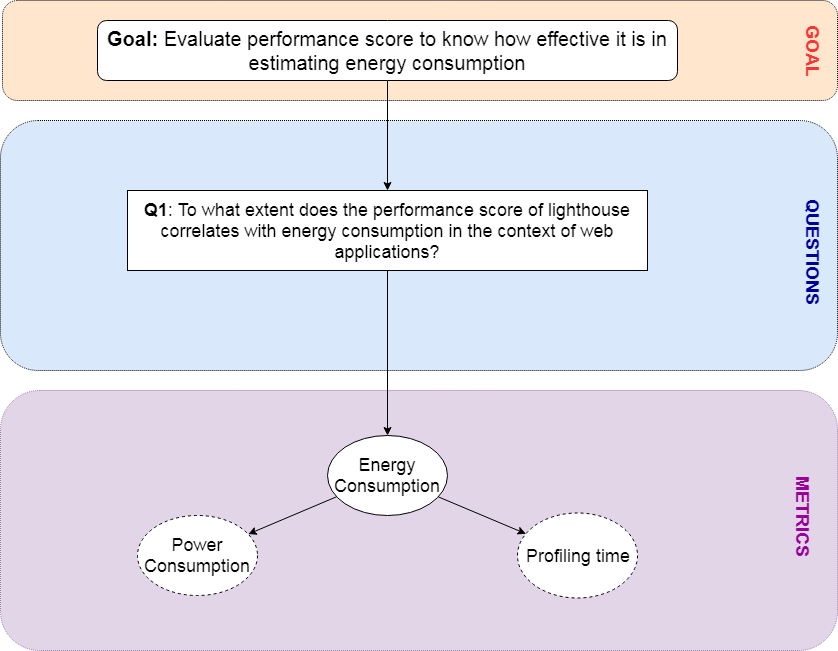
\includegraphics[width=\linewidth]{./Images/GQM.png}
  \caption{GQM tree of the Experiment}
  \label{fig:GQM}
\end{figure}



